\documentclass[a4paper,12pt]{article} % тип документа

% Поля страниц
\usepackage[left=2.5cm,right=2.5cm,
    top=2cm,bottom=2cm,bindingoffset=0cm]{geometry}
    
%Пакет дял таблиц   
\usepackage{multirow} 
    
%Отступ после заголовка    
\usepackage{indentfirst}


% Рисунки
\usepackage{floatrow,graphicx,calc}
\usepackage{wrapfig}

%%% Работа с картинками
\usepackage{graphicx}  % Для вставки рисунков
\graphicspath{{images/}}  % папки с картинками
\setlength\fboxsep{3pt} % Отступ рамки \fbox{} от рисунка
\setlength\fboxrule{1pt} % Толщина линий рамки \fbox{}
\usepackage{wrapfig} % Обтекание рисунков и таблиц текстом

% Создаём новый разделитель
\DeclareFloatSeparators{mysep}{\hspace{1cm}}

% Ссылки?
\usepackage{hyperref}
\usepackage[rgb]{xcolor}
\hypersetup{				% Гиперссылки
    colorlinks=true,       	% false: ссылки в рамках
	urlcolor=blue          % на URL
}


%  Русский язык
\usepackage[T2A]{fontenc}			% кодировка
\usepackage[utf8]{inputenc}			% кодировка исходного текста
\usepackage[english,russian]{babel}	% локализация и переносы

% Математика
\usepackage{amsmath,amsfonts,amssymb,amsthm,mathtools}

%%% Дополнительная работа с математикой
\usepackage{amsmath,amsfonts,amssymb,amsthm,mathtools} % AMS
\usepackage{icomma} % "Умная" запятая: $0,2$ --- число, $0, 2$ --- перечисление

% Что-то 
\usepackage{wasysym}


\begin{document}
\begin{center}
	\footnotesize{ФЕДЕРАЛЬНОЕ ГОСУДАРСТВЕННОЕ АВТОНОМНОЕ ОБРАЗОВАТЕЛЬНОЕ 			УЧРЕЖДЕНИЕ ВЫСШЕГО ОБРАЗОВАНИЯ}\\
	\footnotesize{МОСКОВСКИЙ ФИЗИКО-ТЕХНИЧЕСКИЙ ИНСТИТУТ\\(НАЦИОНАЛЬНЫЙ 			ИССЛЕДОВАТЕЛЬСКИЙ УНИВЕРСИТЕТ)}\\
	\footnotesize{ФИЗТЕХ-ШКОЛА ФИЗИКИ И ИССЛЕДОВАНИЙ им. ЛАНДАУ\\}
	\hfill \break
	\hfill \break
	\hfill \break
	\hfill \break
\end{center}

\begin{center}   
    \hfill \break
	\hfill \break
	\hfill \break
	\hfill \break    \hfill \break
	\hfill \break
	\hfill \break
	\hfill \break
    \hfill \break
    \hfill \break
	\hfill \break
	\large{Лабораторная работа № 2.2.6 \\\textbf{Определение энергии активации
	по температурной зависимости вязкости жидкости}}\\
	\begin{flushright}
		Плотникова Анастасия Александровна\\
		Группа Б02-406
	\end{flushright}
	\hfill \break
	\hfill \break
	\hfill \break
\end{center}
\hfill \break
\hfill \break
\hfill \break
\hfill \break
\hfill \break
\hfill \break
\hfill \break
\hfill \break
\hfill \break
\hfill \break
\hfill \break
\hfill \break
\hfill \break
\begin{center}
	Долгопрудный, 2025 г.
\end{center}
\thispagestyle{empty}
\newpage
	\textbf{Цель работы:}\\ 
	1) измерение скорости падения шариков при разной температуре жидкости; \\
	2) вычисление вязкости жидкости по закону Стокса и расчёт энергии активации. \\
	\hfill \break
	
	\textbf{В работе используются:}\\ 
	стеклянный цилиндр с исследуемой жидкостью (глицерин); \\
	мелкие шарики (диаметром порядка 1 мм); \\
	микроскоп отсчетный МПБ-2 ($\sigma = 0.05$ мм); \\
	термостат Julabo CORIOCD-B17: 	\par
	погрешность поддержания температуры: $dT = 0.03 \, K$; \\
	секундомер. \\

\section*{Теоретическая справка}

\medskip 

\subsection*{Энергия активации и температурная зависимость вязкости}
В жидкости присутствует ближний, но не дальний порядок.

Для того чтобы перейти в новое состояние, тепловая энергия молекул должна — вследствие флуктуации — увеличиться на некоторую величину W, называемую \textit{энергией активации}.

\medskip

Вязкость жидкости экспоненциально зависит от температуры, что описывается формулой Больцмана:
\begin{equation}
    \eta \sim A e^{W/kT},
\end{equation}
где $\eta$ — вязкость, \\
$W$ — энергия активации, \\
$k$ — постоянная Больцмана, \\
$T$ — температура.

Графически зависимость $\ln \eta$ от $1/T$ представляет собой прямую линию, угловой коэффициент которой позволяет определить $W$:
\begin{equation}
    W = -k \frac{d(\ln \eta)}{d(1/T)}
		\label{W}
\end{equation}

\subsection*{Закон Стокса}
Сила сопротивления, действующая на шарик в вязкой жидкости, выражается через закон Стокса:
\begin{equation}
    F = 6\pi \eta r v,
\end{equation}
где $r$ — радиус шарика, \\
$v$ — его скорость.

При установившемся движении шарика баланс сил записывается как:
\begin{equation}
    V g(\rho - \rho_\text{ж}) - 6 \pi \eta r v = V \rho \frac{d v}{d t}
\end{equation}
\begin{equation}
	v(t) = v_\text{уст} - [v_\text{уст} - v(0)]e^{-t/\tau}
\end{equation}
\begin{equation}
	v_{уст} = \frac{Vg (\rho - \rho_\text{ж})}{6 \pi \eta r} = \frac{2}{9} \frac{g r^2 (\rho - \rho_\text{ж})}{\eta}
\end{equation}

Время релаксации:
\begin{equation}
	\tau = \frac{V \rho}{6 \pi \eta r} = \frac{2}{9} \frac{r^2 \rho}{\eta}
	\label{tau}
\end{equation}

Отсюда получаем выражение для вязкости жидкости:
\begin{equation}
    \eta = \frac{2}{9} g r^2 \frac{\rho - \rho_\text{ж}}{v}
		\label{eta}
\end{equation}
 
\subsection*{Число Рейнольдса}
Для проверки применимости закона Стокса вычисляется число Рейнольдса:
\begin{equation}
    Re = \frac{\rho_\text{ж} v r}{\eta}
		\label{Re}
\end{equation}

При $Re < 0.5$ течение считается ламинарным, и формула Стокса применима.

\section*{Экспериментальная установка}

Схема установки изображена на рисунке (\ref{fig:setup}). 

\begin{figure}[h!]
	\centering
	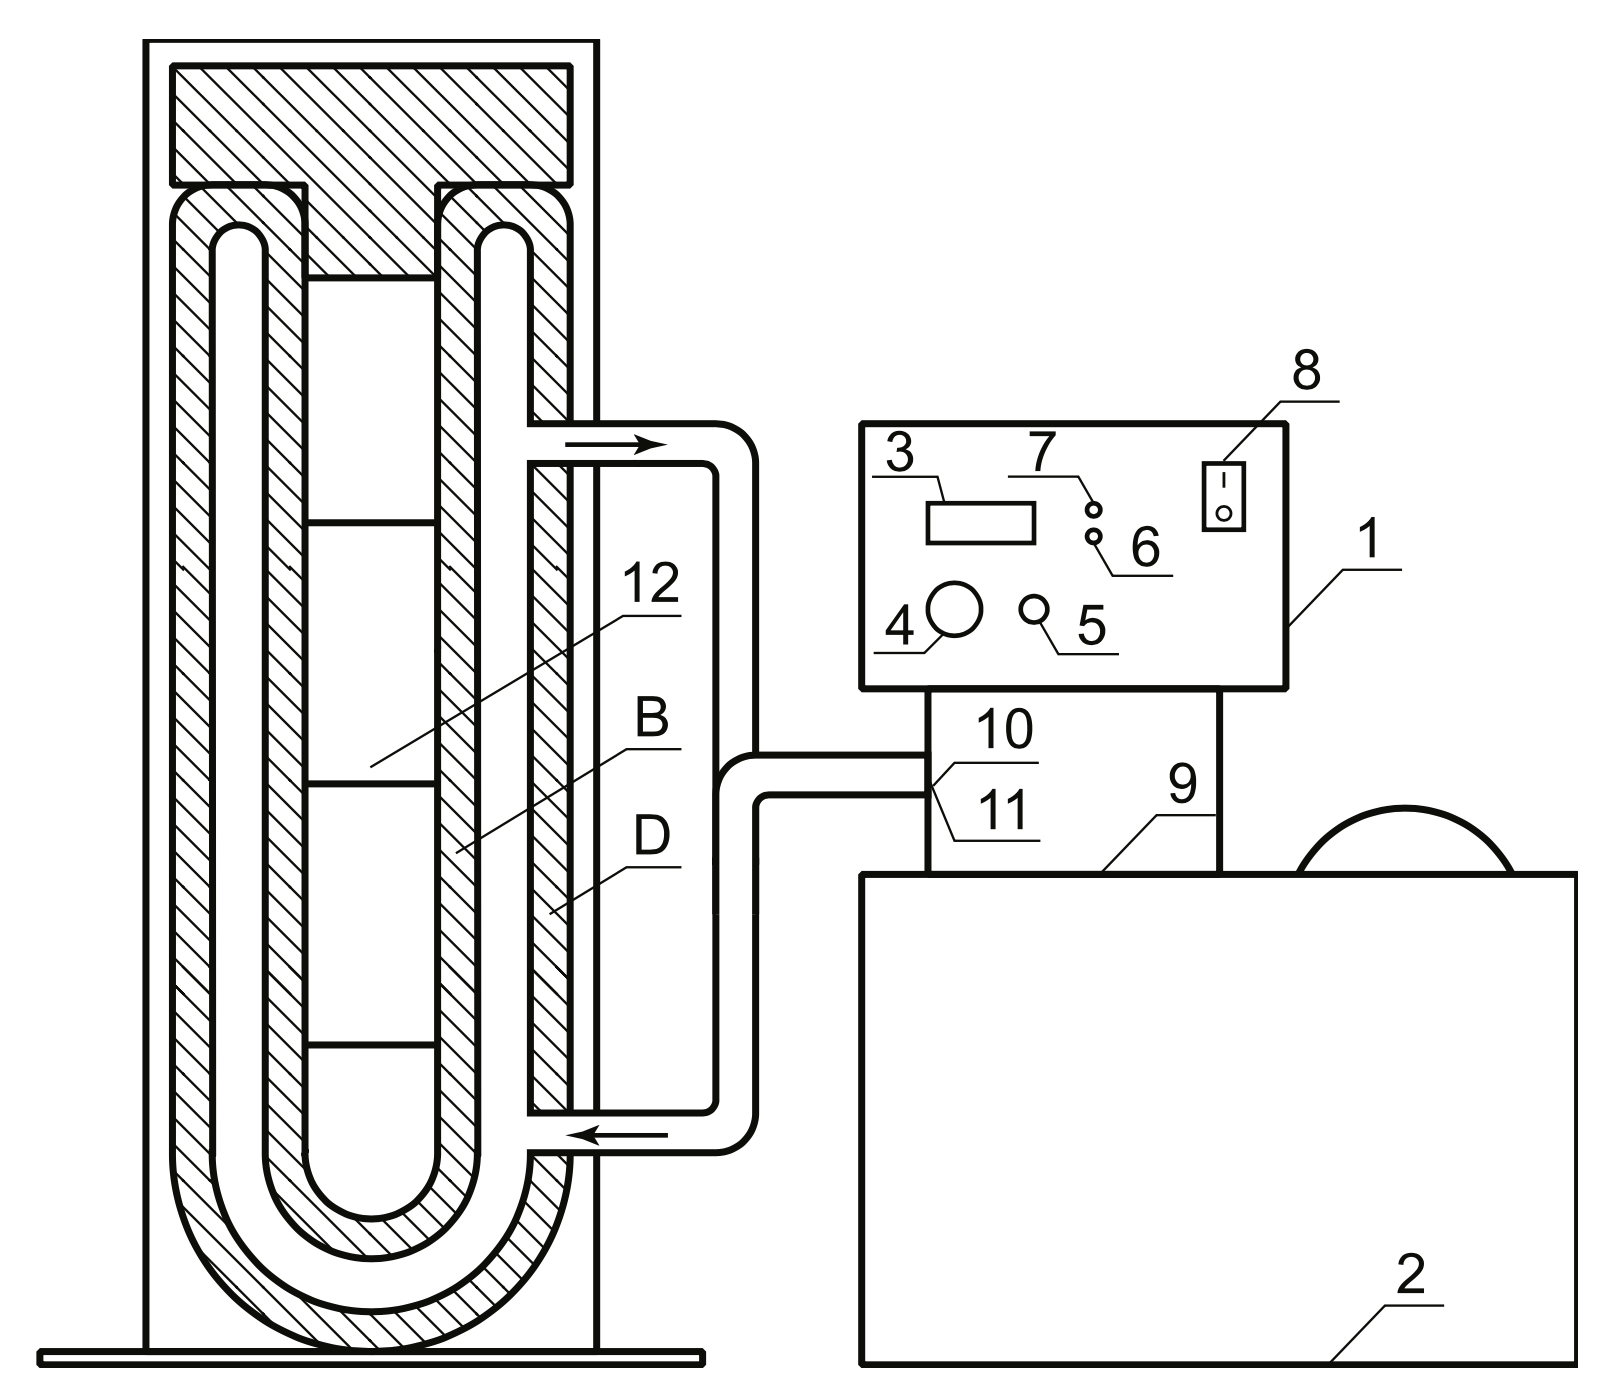
\includegraphics[scale = 0.3]{setup.png}
	\caption{Установка для определения коэффициента вязкости жидкости}
	\label{fig:setup}
\end{figure}

Сосуд помещён в термостат с циркуляцией воды для поддержания постоянной температуры. Температура жидкости контролируется термостатом с точностью до $\pm 0.1$°C. Измерения проводятся при различных температурах от комнатной до 50–60°C.

Радиусы шариков измеряются с помощью горизонтального компаратора или микроскопа. Для каждого шарика вычисляется среднее значение диаметра. Плотность шариков определяется по справочным таблицам, а плотность исследуемой жидкости — по графику зависимости $\rho_{ж}(T)$.

Термостат оборудован цифровым индикатором температуры, системой циркуляции жидкости и нагревателем. Регулировка температуры осуществляется с помощью ручки настройки. Включение нагрева и достижение установленной температуры сопровождаются светодиодными индикаторами.

Схема устройства термостата изображена на рисунке (\ref{fig:thermostat}).

\begin{figure}[h!]
	\centering
	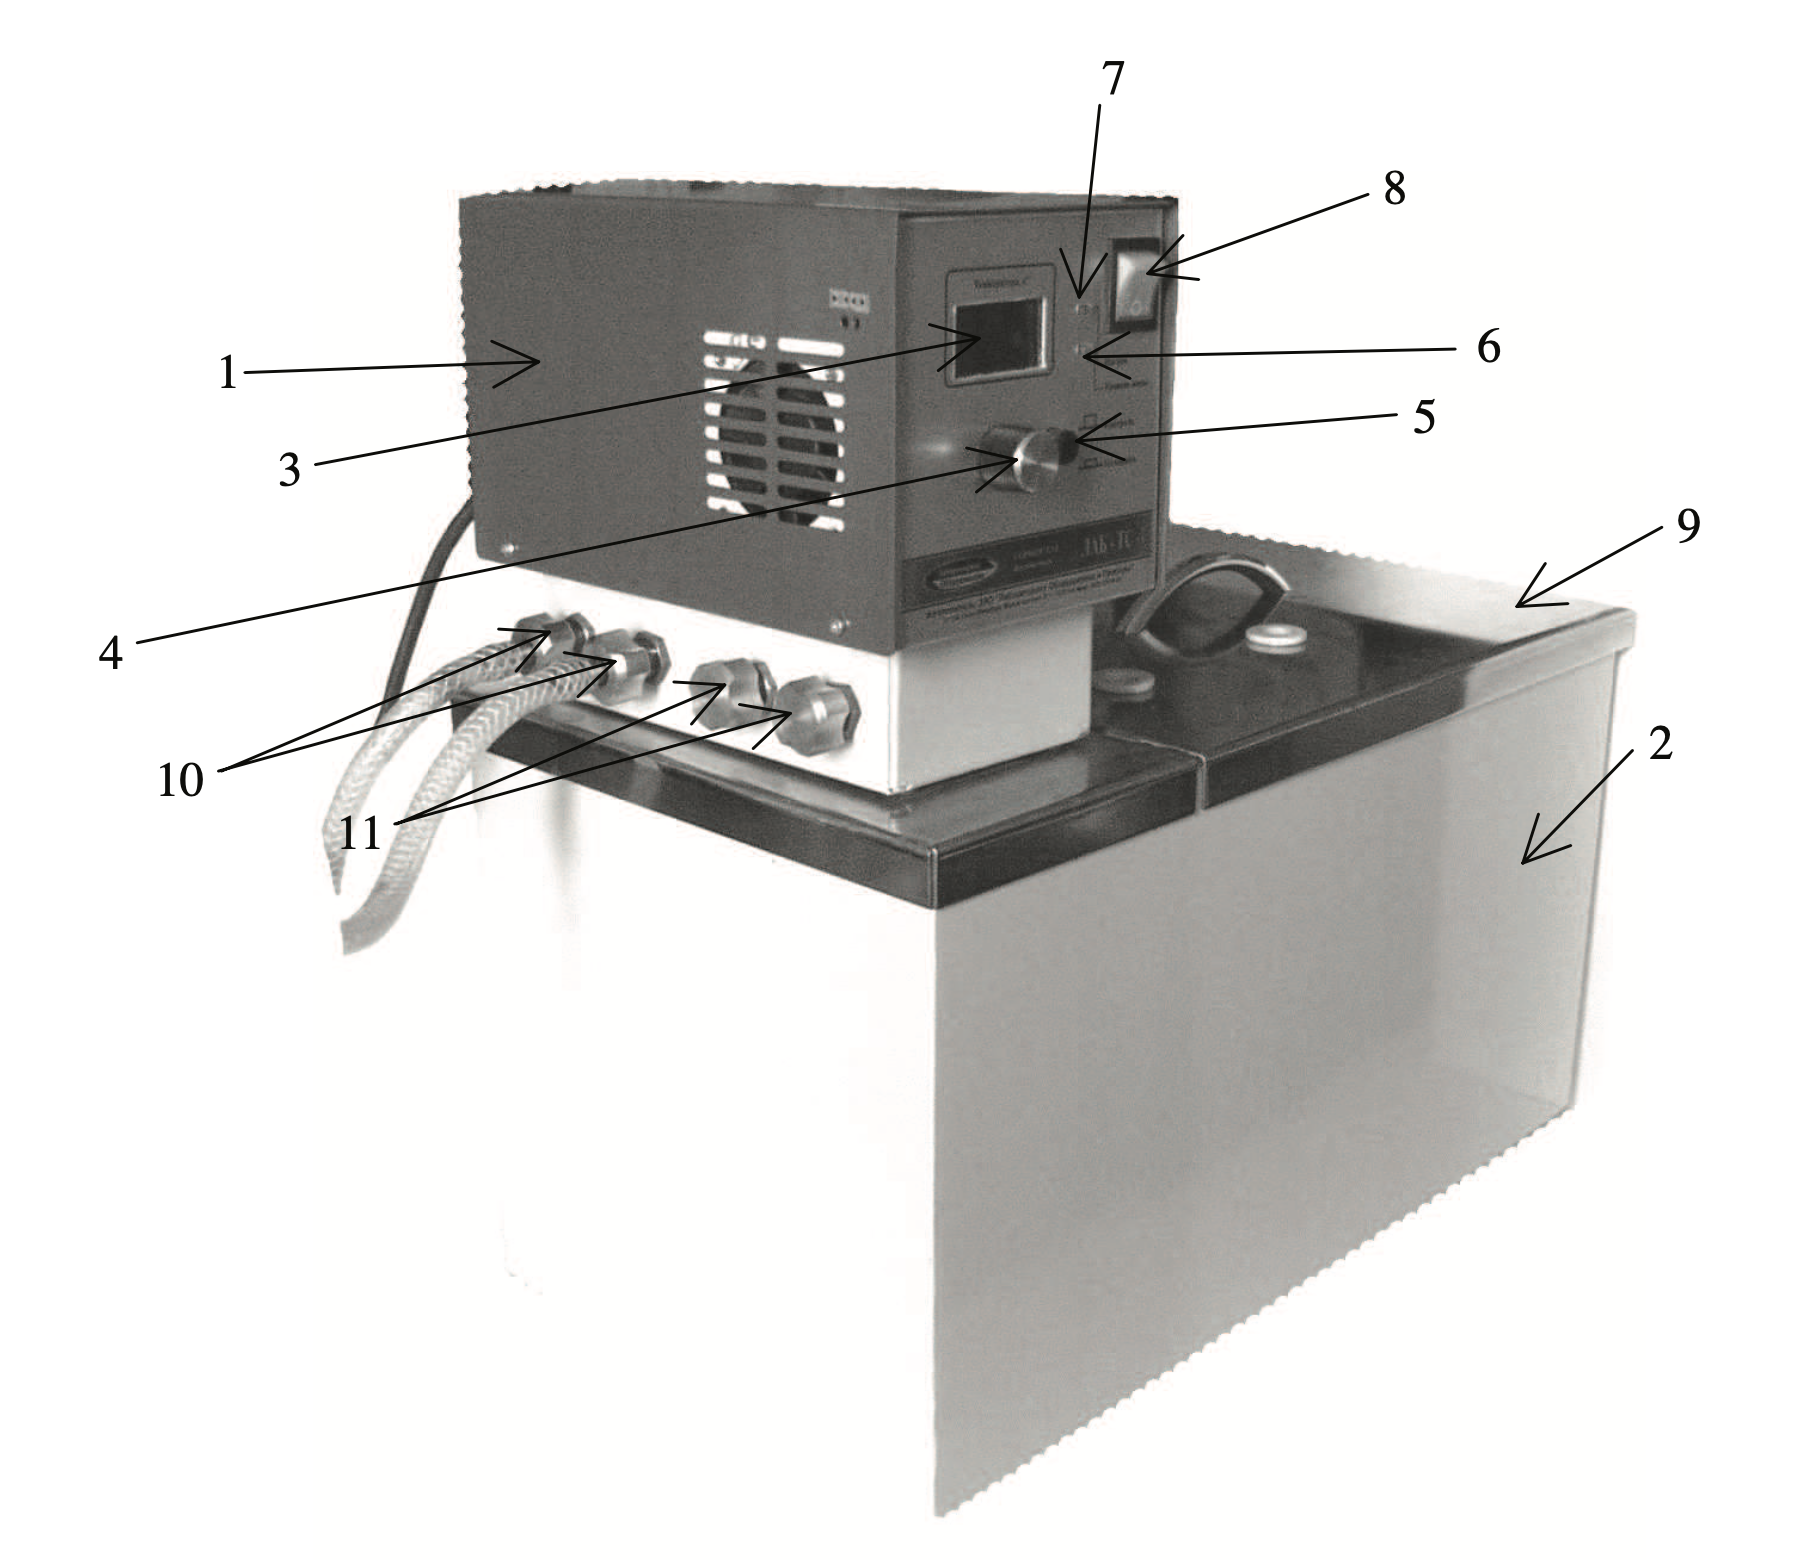
\includegraphics[scale = 0.3]{thermostat.png}
	\caption{Устройство термостата}
	\label{fig:thermostat}
\end{figure}

Опыт по измерению скорости падения шариков проводится после установления термического равновесия системы. Для каждого значения температуры выполняются несколько измерений с шариками различного диаметра.


\section*{Ход работы}

\begin{enumerate}
  \item Перед началом работы зафиксируем плотности материалов шариков и внутренний диаметр сосуда, в который мы намереваемся их бросать.
	\begin{equation}
		\rho_\text{ст} = (2.5 \pm 0.1) \, \text{г/см}^3, \qquad \rho_\text{м} = (7.8 \pm 0.1) \, \text{г/см}^3
	\end{equation}

	Внутренний диаметр измерим два раза, рассчитаем погрешности.
	\begin{equation}
		D = 2R = (2.5 \pm 0.2) \, \text{см}
	\end{equation}
	
	Для каждого из материалов отберём $16$ шариков различного размера и с помощью микроскопа измерим их средние диаметры. Будем измерять по 4 шарика каждого материала по ходу работы. Диаметр стеклянных шариков измеряем дважды, а металлические (предположительно, стальные) — трижды, меняя их ориентацию относительно микроскопа. Результаты занесем в таблицу (\ref{tab:balls}).
  
	\begin{table}[h!]
    \centering
    \begin{tabular}{|c|cc|c|c|ccc|c|}
			\hline
			$N_{\text{ст}}$ & $d_1^{\text{ст}},$ мм & $d_2^{\text{ст}},$ мм & $d^{\text{ст}},$ мм & $N_{\text{м}}$ & $d_1^{\text{м}},$ мм & $d_2^{\text{м}},$ мм & $d_3^{\text{м}},$ мм & $d^{\text{м}},$ мм \\
			\hline
			11 & 2,05 & 2,00 & 2,03 & 16 & 0,80 & 0,80 & 0,75 & 0,78 \\
			12 & 2,00 & 2,10 & 2,05 & 17 & 0,75 & 0,75 & 0,75 & 0,75 \\
			13 & 2,10 & 2,15 & 2,13 & 18 & 0,75 & 0,70 & 0,75 & 0,73 \\
			14 & 2,00 & 2,10 & 2,05 & 19 & 0,75 & 0,75 & 0,75 & 0,75 \\
			21 & 2,10 & 2,10 & 2,10 & 26 & 0,75 & 0,75 & 0,80 & 0,77 \\
			22 & 2,15 & 2,15 & 2,15 & 27 & 0,65 & 0,60 & 0,65 & 0,63 \\
			23 & 2,10 & 2,10 & 2,10 & 28 & 0,80 & 0,75 & 0,75 & 0,77 \\
			24 & 2,10 & 2,15 & 2,13 & 29 & 0,65 & 0,60 & 0,65 & 0,63 \\
			31 & 2,00 & 2,00 & 2,00 & 36 & 0,85 & 0,80 & 0,90 & 0,85 \\
			32 & 2,10 & 2,05 & 2,08 & 37 & 0,75 & 0,75 & 0,70 & 0,73 \\
			33 & 2,10 & 2,00 & 2,05 & 38 & 0,80 & 0,75 & 0,75 & 0,77 \\
			34 & 2,00 & 2,05 & 2,03 & 39 & 0,70 & 0,65 & 0,70 & 0,68 \\
			41 & 2,15 & 2,15 & 2,15 & 46 & 0,75 & 0,80 & 0,75 & 0,77 \\
			42 & 2,10 & 2,10 & 2,10 & 47 & 0,80 & 0,70 & 0,75 & 0,75 \\
			45 & 2,10 & 2,10 & 2,10 & 48 & 0,80 & 0,75 & 0,75 & 0,77 \\
			50 & 2,10 & 2,15 & 2,13 & 49 & 0,80 & 0,80 & 0,75 & 0,78 \\
			\hline
    \end{tabular}
    \caption{Значения диаметров стеклянных и металлических шариков}
    \label{tab:balls}
	\end{table}

  \item Измерим установившиеся скорости падения шариков и вычислите вязкость $\eta$ по формуле (\ref{eta}). 
	
	За начало отсчета возьмем момент прохождения шариком верхней риски на сосуде, а в качестве времен $t_1$ и $t_2$ — моменты прохождения шариком средней и нижней рисок. Расстояния между соседними рисками: $l = (10.0 \pm 0.1)$ см (измерено дважды). 
	
	Измерения выполним для $8$ значений температуры в интервале $25-60 ^\circ C$. Значения представлены в таблицах (\ref{tab:glass_times}) и (\ref{tab:metal_times}) для стеклянных и металлических шариков, соответственно.
  
	После каждого погружения шарика в глицерин будем сразу закрывать крышку. Вязкость воды в тысячи раз меньше вязкости глицерина, поэтому следует минимизировать её возможное влияние, то есть попадание водяных паров.

	Для каждого значения температуры определим плотность жидкости $\rho_\text{ж}$ по графику $\rho_\text{ж} (T)$, изображенного на рисунке (\ref{fig:rho_T}). 

	\begin{figure}[h!]
		\centering
		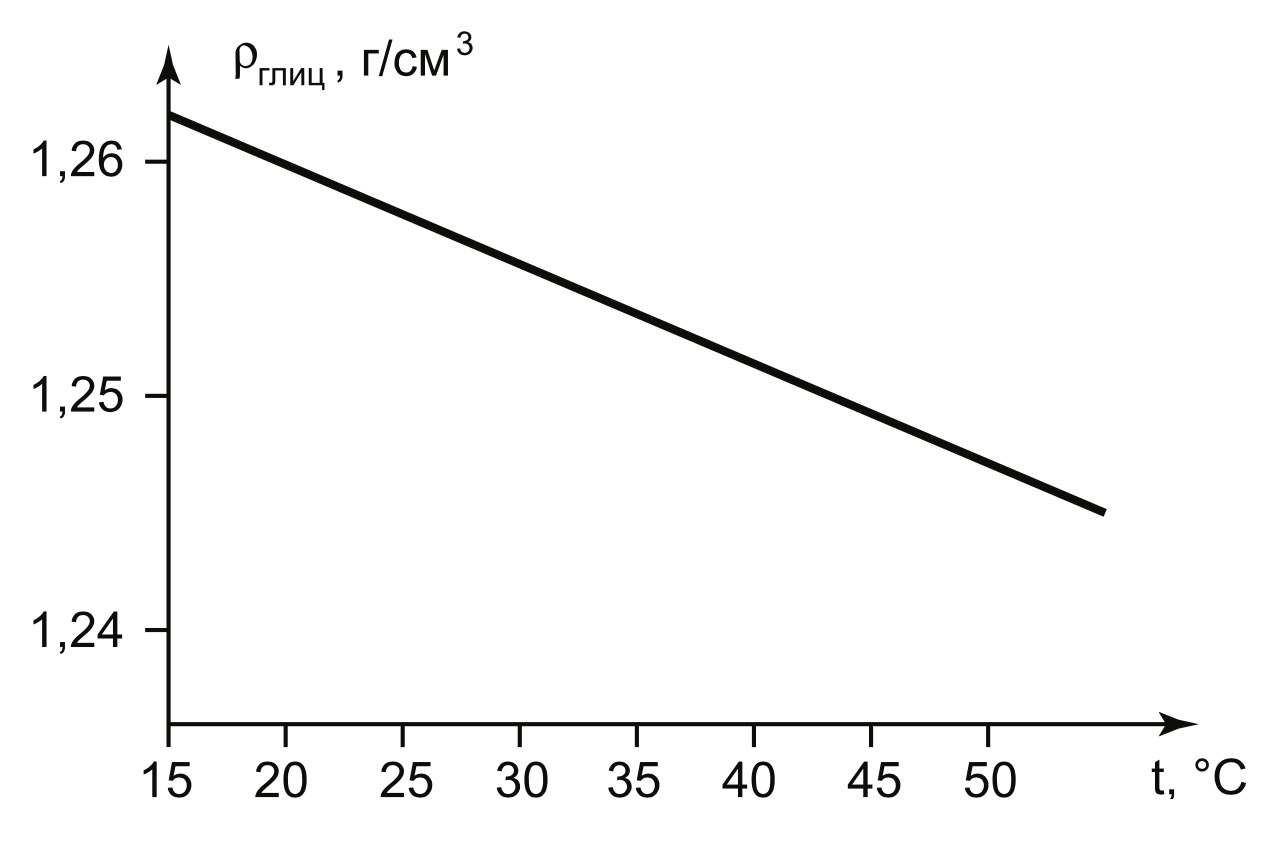
\includegraphics[scale = 0.35]{rho_t.png}
		\caption{Зависимость плотности глицерина от температуры}
		\label{fig:rho_T}
	\end{figure}
	
	Их значения также представлены в таблицах (\ref{tab:glass_times}) и (\ref{tab:metal_times}).

	\begin{table}[h!]
		\centering
		\begin{tabular}{|c|c|c|cc|cc|c|c|c|}
			\hline
			$T, \, ^\circ C$ & $\rho_\text{ж}, \frac{\text{г}}{\text{см}}^3$ & $N_{\text{ст}}$ & $t_1, c$ & $t_2, c$ & $v_1$, см/с & $v_2$, см/с & $v$, см/с & $\eta, 10^{-1}, \frac{\text{кг}}{\text{м·с}}$ & $\ln(\eta)$ \\
			\hline
			25.01 & 1.258 & 11 & 21.78 & 43.73 & 0.4591 & 0.4574 & 0.458 $\pm$ 0.004 & 6.0576 & -0,4841 \\
						&      & 12 & 22.05 & 44.01 & 0.4535 & 0.4544 & 0.454 $\pm$ 0.004 & 6.2664 &        \\
			30.15 & 1.256 & 13 & 15.73 & 30.40 & 0.6357 & 0.6579 & 0.647 $\pm$ 0.012 & 4.7341 & -0,7910 \\
						&      & 14 & 15.17 & 30.48 & 0.6592 & 0.6562 & 0.658 $\pm$ 0.006 & 4.3330 &        \\
			34.95 & 1.254 & 21 & 9.82  & 19.87 & 1.0183 & 1.0065 & 1.012 $\pm$ 0.012 & 2.9585 & -1,1745 \\
						&      & 22 & 10.26 & 20.51 & 0.9747 & 0.9751 & 0.975 $\pm$ 0.010& 3.2204 &        \\
			39.91 & 1.252 & 23 & 7.64  & 15.12 & 1.3089 & 1.3228 & 1.316 $\pm$ 0.018& 2.2801 & -1,4642 \\
						&      & 24 & 7.60  & 15.33 & 1.3158 & 1.3046 & 1.310 $\pm$ 0.017 & 2.3447 &        \\
			44.90 & 1.250 & 31 & 5.50  & 10.98 & 1.8182 & 1.8215 & 1.82 $\pm$ 0.03& 1.4978 & -1,8750 \\
						&      & 32 & 5.36  & 10.67 & 1.8657 & 1.8744 & 1.87 $\pm$ 0.03 & 1.5690 &        \\
			50.13 & 1.247 & 33 & 4.50  & 9.03  & 2.2222 & 2.2148 & 2.22 $\pm$ 0.04 & 1.2931 & -2,0702 \\
						&      & 34 & 4.34  & 8.90  & 2.3041 & 2.2472 & 2.28 $\pm$ 0.05 & 1.2301 &        \\
			55.30 & 1.245 & 41 & 2.91  & 5.98  & 3.4364 & 3.3445 & 3.4 $\pm$ 0.1 & 0.9323 & -2,3745 \\
						&      & 42 & 3.07  & 6.18  & 3.2573 & 3.2362 & 3.25 $\pm$ 0.08 & 0.9288 &        \\
			60.57 & 1.243 & 45 & 2.28  & 4.83  & 4.3860 & 4.1408 & 4.3 $\pm$ 0.2 & 0.7086 & -2,6220 \\
						&      & 50 & 2.39  & 4.83  & 4.1841 & 4.1408 & 4.16 $\pm$ 0.14 & 0.7431 &        \\
			\hline
		\end{tabular}
		\caption{Значения $t$, $v$, $\eta$, $\ln(\eta)$ для стеклянных шариков}
		\label{tab:glass_times}
	\end{table}

	\begin{table}[h!]
		\centering
		\begin{tabular}{|c|c|c|cc|cc|c|c|c|}
			\hline
			$T, \, ^\circ C$ & $\rho_\text{ж}, \frac{\text{г}}{\text{см}}^3$ & $N_{\text{м}}$ & $t_1, c$ & $t_2, c$ & $v_1$, см/с & $v_2$, см/с & $v$, см/с & $\eta, 10^{-1}, \frac{\text{кг}}{\text{м·с}}$ & $\ln(\eta)$ \\
			\hline
			25.01 & 1.258 & 16 & 30.4  & 60.48 & 0.329  & 0.331  & 0.330 $\pm$ 0.003 & 6.6333 & -0,4108 \\
						&      & 17 & 33.1  & 65.99 & 0.302  & 0.303  & 0.303 $\pm$ 0.002 & 6.6279 &        \\
			30.15 & 1.256 & 18 & 23.95 & 47.55 & 0.418  & 0.421  & 0.419 $\pm$ 0.004 & 4.5769 & -0,7388 \\
						&      & 19 & 24.82 & 49.58 & 0.403  & 0.403  & 0.403 $\pm$ 0.003 & 4.9764 &        \\
			34.95 & 1.254 & 26 & 12.38 & 24.22 & 0.808  & 0.826  & 0.817 $\pm$ 0.012 & 2.5675 & -1,2733 \\
						&      & 27 & 21.29 & 42.13 & 0.470  & 0.475  & 0.472 $\pm$ 0.005 & 3.0305 &        \\
			39.91 & 1.252 & 28 & 10.76 & 21.49 & 0.929  & 0.931  & 0.93 $\pm$ 0.01 & 2.2555 & -1,7794 \\
						&      & 29 & 7.83  & 15.61 & 1.277  & 1.281  & 1.28 $\pm$ 0.02 & 1.1191 &        \\
			44.90 & 1.250 & 36 & 6.55  & 12.47 & 1.527  & 1.604  & 1.57 $\pm$ 0.05 & 1.6478 & -1,8173 \\
						&      & 7  & 8.48  & 16.41 & 1.179  & 1.219  & 1.20 $\pm$ 0.02  & 1.6012 &        \\
			50.13 & 1.247 & 38 & 5.24  & 10.6  & 1.908  & 1.887  & 1.90 $\pm$ 0.03 & 1.1062 & -2,1536 \\
						&      & 39 & 7.21  & 14.73 & 1.387  & 1.358  & 1.37 $\pm$ 0.02  & 1.2151 &        \\
			55.30 & 1.245 & 46 & 4.14  & 8.34  & 2.415  & 2.398  & 2.41 $\pm$ 0.05  & 0.8724 & -2,4402 \\
						&      & 47 & 4.28  & 8.77  & 2.336  & 2.281  & 2.31 $\pm$ 0.05  & 0.8705 &        \\
			60.57 & 1.243 & 48 & 3.23  & 6.37  & 3.096  & 3.140  & 3.12 $\pm$ 0.08  & 0.6737 & -2,6734 \\
						&      & 49 & 3.22  & 6.45  & 3.106  & 3.101  & 3.10 $\pm$ 0.08  & 0.7066 &        \\
			\hline
		\end{tabular}
		\caption{Значения $t$, $v$, $\eta$, $\ln(\eta)$ для металлических шариков}
		\label{tab:metal_times}
	\end{table}
  
  \item Для каждого из опытов вычислим значение числа Рейнольдса $Re$ (\ref{Re}), оценим время релаксации $\tau$ (\ref{tau}) и путь релаксации $S = v_\text{уст} \tau$. Результаты в таблице (\ref{tab:ReTauS}). 
  
	\begin{table}[h!]
    \centering
    \begin{tabular}{|c|c|c|c||c|c|c|}
			\hline
			& \multicolumn{3}{c||}{Стекло} & \multicolumn{3}{c|}{Металл} \\
			\hline
			$T, \, ^\circ C$ & Re, 1 & $\tau, \, 10^{-3}$ c & $S, \, 10^{-6}$ м & Re, 1 & $\tau, \, 10^{-3}$ c & $S, \, 10^{-6}$ м \\
			\hline
			25,01 & 0,232 & 0,945 & 4,292 & 0,144 & 0,363 & 1,098 \\
			30,15 & 0,455 & 1,285 & 8,451 & 0,265 & 0,504 & 2,030 \\
			34,95 & 0,989 & 1,886 & 18,383 & 0,529 & 0,859 & 4,058 \\
			39,91 & 1,773 & 2,519 & 33,007 & 2,372 & 1,425 & 18,234 \\
			44,90 & 3,810 & 3,799 & 71,043 & 2,306 & 1,481 & 17,752 \\
			50,13 & 5,625 & 4,618 & 105,079 & 3,688 & 2,072 & 28,439 \\
			55,30 & 10,862 & 6,260 & 203,254 & 8,247 & 2,760 & 63,712 \\
			60,57 & 17,821 & 8,026 & 334,062 & 13,974 & 3,485 & 108,144 \\
			\hline
    \end{tabular}
    \caption{Значения $Re$, $\tau$, $S$ для стеклянных и металлических шариков}
    \label{tab:ReTauS}
	\end{table}	

	Проанализируем применимость формулы Стокса в каждом эксперименте. То есть проверим, что: \\
	1) течение ламинарно ($Re < 1$); \\
	2) скорость движения шара установилась; \\
	3) жидкость однородная и несжимаемая; \\
	4) влияние стенок сосуда отсутствуют. 

	Условия 2–3 выполнены в каждом из экспериментов. Условие 4 не выполняется при одном из запусков металлического шарика при $t = 44.90 \, ^\circ C$ — он проходит слишком близко к стенке. Влияние заметно на графике: небольшой выброс.

	Условия 1 выполняется в диапазоне температур $25 – 35 \, ^\circ C$. Поэтому для более высоких температур формула Стокса неприменима.
  
  \item Построим график зависимости $\ln \eta$ от $1/T$ (см. рис. (\ref{fig:eta1T})).
  
	\begin{figure}[h]
		\centering
		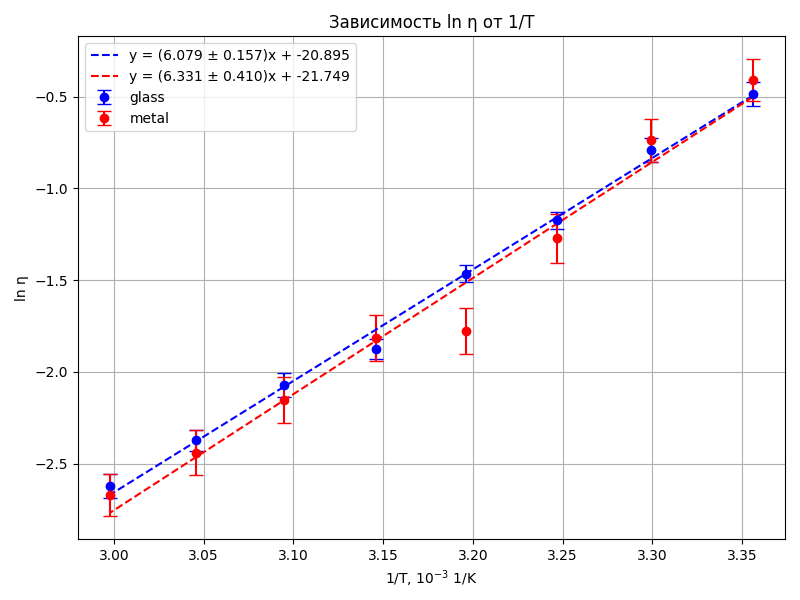
\includegraphics[scale = 0.75]{graph.png}
		\caption{График зависимости $\ln \eta$ от $1/T$}
		\label{fig:eta1T}
	\end{figure}
  
	Для определения углового коэффициента воспользуемся методом наименьших квадратов. 
	\begin{equation}
		k^\text{ст/м} = \frac{\sum_{i=1}^{n} \left(\frac{1}{T_i} - \langle \frac{1}{T} \rangle \right) \left(\ln(\eta_i) - \langle \ln(\eta) \rangle \right)}{\sum_{i=1}^{n} \left(\frac{1}{T_i} - \langle \frac{1}{T} \rangle \right)^2}
	\end{equation}
	\begin{equation}
		\sigma_{k^\text{ст/м}} = \sqrt{\frac{1}{n-2} \cdot \frac{\sum_{i=1}^{n} \left( \ln(\eta_i) - \hat{\ln(\eta_i)} \right)^2}{\sum_{i=1}^{n} \left( \frac{1}{T_i} - \langle \frac{1}{T} \rangle \right)^2}}
	\end{equation}	
  \item По угловому коэффициенту прямой $\ln \eta (1/T)$ с помощью формулы (\ref{W}) определим энергию активации. 
  
	\begin{equation}
		k^{\text{ст}} = 6.079 \cdot 10^{3} \, K, \qquad k^{\text{м}} = 6.331 \cdot 10^{3} \, K
	\end{equation}
	\begin{equation}
		\sigma_{k^{\text{ст}}_\text{МНК}} = 0.16 \cdot 10^{-3} \, K, \qquad \sigma_{k^{\text{м}}_\text{МНК}} = 0.41 \cdot 10^{-3} \, K
	\end{equation}

	Рассчитаем погрешности прямых измерений.
	\begin{equation}
		\sigma_k = \sqrt{\left( \frac{\partial k}{\partial \eta} \sigma_{\eta} \right)^2 + \left( \frac{\partial k}{\partial T} \sigma_T \right)^2} = \sqrt{\frac{\sigma_{\eta}^2}{T^2} + \frac{(\ln \eta)^2 \sigma_T^2}{T^4}}
	\end{equation}
	\begin{align}
		\sigma_\eta &= \sqrt{\left( \frac{\partial \eta}{\partial r} \sigma_r \right)^2 + \left( \frac{\partial \eta}{\partial \Delta \rho} \sigma_{\Delta \rho} \right)^2 + \left( \frac{\partial \eta}{\partial v} \sigma_v \right)^2} = \\
		&= \sqrt{\left( \frac{2r \Delta \rho}{v} \sigma_r \right)^2 + \left( \frac{r^2}{v} \sigma_{\Delta \rho} \right)^2 + \left( -\frac{r^2 \Delta \rho}{v^2} \sigma_v \right)^2}
	\end{align}
	\begin{equation}
		\sigma_r = \sqrt{\sigma_{r_\text{случ}}^2 + \sigma_{r_\text{приб}}^2}
	\end{equation}
	\begin{equation}
		\sigma_{\Delta \rho} = \sqrt{\sigma_{\rho}^2 + \sigma_{\rho_{\text{ж}}}^2} 
	\end{equation}
	\begin{equation}
		\sigma_v = \sqrt{\sigma_{v_\text{случ}}^2 + \sigma_{v\text{приб}}^2} = \sqrt{\sigma_{v_\text{случ}}^2 + v^2 (\frac{\sigma_l}{l}^2 + \frac{\sigma_t}{t}^2)}
	\end{equation}
	При расчете погрешности времени учитываем скорость реакции человека: 
	\begin{equation}
		\sigma_t^\text{реакции} = 0.3 \cdot 2 = 0.6 \, c
	\end{equation}
	

	Вернемся к нашим баранам.
	\begin{equation}
		W^{\text{ст/м}} = k \frac{d(\ln \eta)}{d(1/T)} = k \cdot k^{\text{ст/м}}
	\end{equation}
	Постоянную Больцмана, как и все константы, мы возьмем с достаточной точностью. Поэтому $\varepsilon_W = \varepsilon_k$, где k — соответствующий угловой коэффициент.

	Аккуратно рассчитаем все погрешности по формулам выше. Вычислим значения $W^{\text{ст}}$ и $W^{\text{м}}$.

	\begin{equation}
		W^{\text{ст}} = k \cdot k^{\text{ст}} = (8.4 \pm 1.2) \cdot 10^{-20} \, \text{Дж}
		\label{W1}
	\end{equation}
	\begin{equation}
		W^{\text{м}} = k \cdot k^{\text{ст}} = (9 \pm 2) \cdot 10^{-20} \, \text{Дж}
		\label{W2}
	\end{equation}

	Результаты совпадают в пределах погрешности.
	
	\item Погрешность полученных результатов оценена выше.
\end{enumerate}

\section*{Вывод}

Все цели работы были достигнуты.

\begin{enumerate}
	\item Скорости падения шариков при разной температуре жидкости измерены. Результаты в таблицах (\ref{tab:glass_times}) и (\ref{tab:metal_times}).
	\item Вязкость глицерина при разных температурах вычислена по формуле Стокса. Результаты в тех же таблицах (\ref{tab:glass_times}) и (\ref{tab:metal_times}). 
	
	Энергия активации также рассчитана (для опытов со стеклянными и металлическими шариками отдельно). Результаты записаны в уравнениях (\ref{W1}) и (\ref{W2}).
\end{enumerate}

\end{document}
